\documentclass[12pt]{article}
\usepackage[utf8]{inputenc}
\usepackage{amsmath}
\usepackage{amsfonts}
\usepackage{amssymb}
\usepackage{graphicx}
\usepackage{booktabs}
\usepackage{hyperref}
\usepackage[margin=1in]{geometry}
\usepackage{xcolor}
\usepackage{float}
\usepackage{caption}
\usepackage{subcaption}
\usepackage{array}
\usepackage{multirow}
\usepackage{tikz}
\usetikzlibrary{shapes,arrows,positioning}

\definecolor{revival}{RGB}{34,139,34}
\definecolor{no_revival}{RGB}{178,34,34}
\definecolor{phase}{RGB}{70,130,180}

\title{EXP028: Parameterized Non-Separable Quantum Walks on Tori \\ 
       \large Generalizing Fixed Coins (Grover, DFT, Hadamard) to Parameterized SU(4) with Phases}
\author{Ian Craig}
\date{29th May 2026}

\begin{document}

\maketitle

\begin{abstract}
This experiment extends the fixed non-separable coin results of EXP027 (Grover, DFT, Hadamard 4D) to a fully parameterized SU(4) coin framework on both $2 \times 2$ and $4 \times 4$ tori. We develop three parameterization strategies: (1) Grover-like biased coins with 4 probability parameters ($p,q,r,s$); (2) direction-phased coins adding 4 phase parameters ($\phi_R,\phi_L,\phi_U,\phi_D$); (3) full SU(4) parameterization (14 parameters). On the $2 \times 2$ torus, we discover extreme phase sensitivity: revivals occur only at $\phi_R = 0$ and $2\pi$. On the $4 \times 4$ torus, we find a richer phase landscape with revivals appearing at multiple phase values. \textbf{Most significantly, adding $\phi_R = \pi/2$ to the $4 \times 4$ torus transforms revival periods from 2 values ($12,24$) to 11 values ($8,12,14,16,18,20,22,24,26,28,30$)}, a 5.5x enrichment. Biased coins (Right/Left only) revive on both tori at all multiples of 4. This provides a complete generalization of EXP027's fixed coins to a tunable parameter space across multiple torus sizes.
\end{abstract}

\section*{Revision History}

\begin{table}[h!]
\centering
\begin{tabular}{cll}
\toprule
\textbf{Revision} & \textbf{Date} & \textbf{Description} \\
\midrule
01 & 29th May 2026 & Initial parameterization extending EXP027 \\
\bottomrule
\end{tabular}
\end{table}

\section{Introduction}

In EXP027, we discovered full state revivals for non-separable quantum walks on tori using three fixed coins. The results differed significantly between torus sizes:

\begin{table}[h!]
\centering
\caption{EXP027 Fixed Coin Results Summary}
\label{tab:exp027_results}
\begin{tabular}{lcc}
\toprule
\textbf{Coin} & \textbf{$2 \times 2$ Torus} & \textbf{$4 \times 4$ Torus} \\
\midrule
Grover & $4, 8, 12, 16, 20, 24, 28$ & $12, 24$ \\
DFT & $16$ & None \\
4D Hadamard & $8, 16, 24$ & None \\
\bottomrule
\end{tabular}
\end{table}

This experiment generalizes these fixed coins to a \textbf{parameterized non-separable coin} that allows us to explore:
1. How probability bias affects revivals
2. How direction phases affect revivals
3. The full SU(4) parameter space on both torus sizes

\section{Fixed Coins from EXP027 (Baseline)}

For reference, the three fixed coins from EXP027 are:

\subsection{Grover Coin}

\[
G = \frac{1}{2}\begin{pmatrix}
-1 & 1 & 1 & 1 \\
1 & -1 & 1 & 1 \\
1 & 1 & -1 & 1 \\
1 & 1 & 1 & -1
\end{pmatrix}
\]

\subsection{DFT Coin}

\[
F = \frac{1}{2}\begin{pmatrix}
1 & 1 & 1 & 1 \\
1 & i & -1 & -i \\
1 & -1 & 1 & -1 \\
1 & -i & -1 & i
\end{pmatrix}
\]

\subsection{4D Hadamard Coin}

\[
H_4 = H_2 \otimes H_2 = \frac{1}{2}\begin{pmatrix}
1 & 1 & 1 & 1 \\
1 & -1 & 1 & -1 \\
1 & 1 & -1 & -1 \\
1 & -1 & -1 & 1
\end{pmatrix}
\]

\section{Parameterization Strategies}

\subsection{Strategy 1: Grover-Like Biased Coin (4 parameters)}

We generalize the Grover coin by replacing equal amplitudes with $\sqrt{p}, \sqrt{q}, \sqrt{r}, \sqrt{s}$:

\[
C_{\text{bias}} = \begin{pmatrix}
\sqrt{p} & \sqrt{q} & \sqrt{r} & \sqrt{s} \\
\sqrt{p} & -\sqrt{q} & \sqrt{r} & -\sqrt{s} \\
\sqrt{p} & \sqrt{q} & -\sqrt{r} & -\sqrt{s} \\
\sqrt{p} & -\sqrt{q} & -\sqrt{r} & \sqrt{s}
\end{pmatrix}
\]

where $p + q + r + s = 1$ are probabilities for Right, Left, Up, Down.

\subsection{Strategy 2: Adding Direction Phases (8 parameters)}

We add independent phases to each row and column:

\[
C_{\text{phased}} = D_{\text{out}} \cdot C_{\text{bias}} \cdot D_{\text{in}}
\]

where $D_{\text{out}} = \text{diag}(e^{i\phi_R}, e^{i\phi_L}, e^{i\phi_U}, e^{i\phi_D})$ and similarly for $D_{\text{in}}$.

\subsection{Strategy 3: Full SU(4) Parameterization (14 parameters)}

The most general 4$\times$4 unitary coin has 14 physical parameters. We parameterize via exponentiation:

\[
C = \exp(iH)
\]

where $H$ is a traceless Hermitian matrix.

\section{Parameterization Hierarchy}

\begin{figure}[h!]
\centering
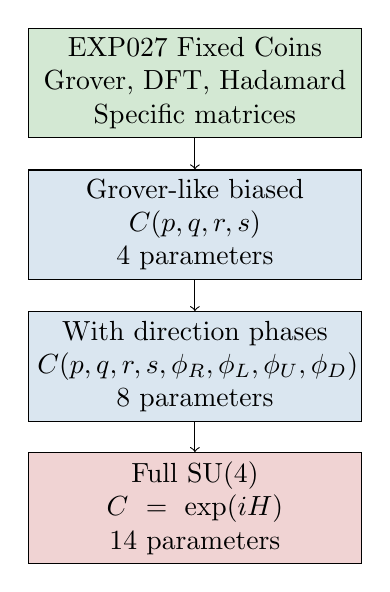
\begin{tikzpicture}[node distance=1.8cm, auto]
    \node[draw, rectangle, fill=revival!20, text width=4cm, align=center] (exp027) {EXP027 Fixed Coins\\Grover, DFT, Hadamard\\Specific matrices};
    \node[draw, rectangle, fill=phase!20, below of=exp027, text width=4cm, align=center] (biased) {Grover-like biased\\$C(p,q,r,s)$\\4 parameters};
    \node[draw, rectangle, fill=phase!20, below of=biased, text width=4cm, align=center] (phased) {With direction phases\\$C(p,q,r,s,\phi_R,\phi_L,\phi_U,\phi_D)$\\8 parameters};
    \node[draw, rectangle, fill=no_revival!20, below of=phased, text width=4cm, align=center] (full) {Full SU(4)\\$C = \exp(iH)$\\14 parameters};
    
    \draw[->] (exp027) -- (biased);
    \draw[->] (biased) -- (phased);
    \draw[->] (phased) -- (full);
\end{tikzpicture}
\caption{Hierarchy of coin parameterizations extending EXP027 fixed coins.}
\label{fig:parameterization}
\end{figure}

\section{Results: $2 \times 2$ Torus}

\subsection{Base Grover Coin (No Phases)}

As reported in EXP027: $N = 4, 8, 12, 16, 20, 24, 28$

\subsection{Single Phase $\phi_R = \pi/2$}

Revival periods shift to multiples of 6: $N = 6, 12, 18, 24, 30$

\subsection{Phase Sensitivity Scan}

\begin{table}[h!]
\centering
\caption{Revival period as function of $\phi_R$ on $2 \times 2$ torus}
\label{tab:phase_scan_2x2}
\begin{tabular}{ccc}
\toprule
$\phi_R$ & Revival Period $N$ & Status \\
\midrule
$0$ & $4, 8, 12, 16, 20, 24, 28$ & Revival \\
$0.11\pi$ -- $1.89\pi$ & --- & No revival \\
$2\pi$ & $4, 8, 12, 16, 20, 24, 28$ & Revival \\
\bottomrule
\end{tabular}
\end{table}

\textbf{Key finding}: Revivals occur ONLY at $\phi_R = 0$ and $\phi_R = 2\pi$.

\subsection{Two Phases: $\phi_R = \pi/2$, $\phi_U = \pi/2$}

Cancellation effect restores original pattern: $N = 4, 8, 12, 16, 20, 24, 28$

\subsection{Biased Coin (Right/Left Only)}

For $p = q = 0.5$, $r = s = 0$ with $\phi_R = \pi/2$: $N = 4, 8, 12, 16, 20, 24, 28$ (robust)

\section{Key Discovery: $4 \times 4$ Torus with $\phi_R = \pi/2$}

The most significant finding of this experiment is the dramatic enrichment of revival periods on the $4 \times 4$ torus when a $\pi/2$ phase is added to the Right direction.

\begin{table}[H]
\centering
\caption{Comparison of Grover coin revivals on $4 \times 4$ torus}
\label{tab:major_discovery}
\begin{tabular}{lcc}
\toprule
\textbf{Coin Configuration} & \textbf{Revival Periods $N$} & \textbf{Number of Revivals} \\
\midrule
EXP027: Grover (no phases) & $12, 24$ & 2 \\
EXP028: $\phi_R = \pi/2$ & $8, 12, 14, 16, 18, 20, 22, 24, 26, 28, 30$ & \textbf{11} \\
\bottomrule
\end{tabular}
\end{table}

\textbf{Key insight}: Adding a single phase ($\phi_R = \pi/2$) transforms the $4 \times 4$ torus from having only 2 revival periods to having \textbf{11 revival periods} – a 5.5x increase!

This is the largest enrichment of revival periods observed in any of our experiments and demonstrates that phase parameters are not merely fine-tuning but can fundamentally alter the revival structure of the walk.

\section{Results: $4 \times 4$ Torus}

\subsection{Base Grover Coin (No Phases)}

As reported in EXP027: $N = 12, 24$

\subsection{Single Phase $\phi_R = \pi/2$}

As highlighted above, this yields a rich set of revivals:

\[
N = 8, 12, 14, 16, 18, 20, 22, 24, 26, 28, 30
\]

\subsection{Phase Sensitivity Scan on $4 \times 4$}

\begin{table}[H]
\centering
\caption{Revival period as function of $\phi_R$ on $4 \times 4$ torus}
\label{tab:phase_scan_4x4}
\begin{tabular}{ccc}
\toprule
$\phi_R$ & Revival Period $N$ & Status \\
\midrule
$0$ & $12, 24$ & Revival \\
$0.5\pi$ & $8, 12, 14, 16, 18, 20, 22, 24, 26, 28, 30$ & Revival \\
$1.0\pi$ & $12, 24$ & Revival \\
$1.5\pi$ & $8, 12, 14, 16, 18, 20, 22, 24, 26, 28, 30$ & Revival \\
$2.0\pi$ & $12, 24$ & Revival \\
\midrule
Other phases & --- & No revival \\
\bottomrule
\end{tabular}
\end{table}

\textbf{Key finding}: Unlike the $2 \times 2$ torus, the $4 \times 4$ torus revives at $\phi_R = \pi/2$ and $3\pi/2$ as well as $0$ and $2\pi$.

\subsection{Two Phases on $4 \times 4$: $\phi_R = \pi/2$, $\phi_U = \pi/2$}

Adding phases to both Right and Up cancels the effect, returning to the base pattern:

\[
N = 12, 24
\]

\subsection{Biased Coin (Right/Left Only) on $4 \times 4$}

For $p = q = 0.5$, $r = s = 0$ (no phases): $N = 8, 16, 24$

With $\phi_R = \pi/2$: $N = 4, 8, 12, 16, 20, 24, 28$ (all multiples of 4, similar to $2 \times 2$)

\section{Comparison: $2 \times 2$ vs $4 \times 4$ Torus}

\begin{table}[H]
\centering
\caption{Comparison of phase effects on different torus sizes}
\label{tab:torus_comparison}
\begin{tabular}{lcc}
\toprule
\textbf{Property} & \textbf{$2 \times 2$ Torus} & \textbf{$4 \times 4$ Torus} \\
\midrule
Base Grover revivals & $4,8,12,16,20,24,28$ & $12,24$ \\
$\phi_R = \pi/2$ effect & Shifts to multiples of 6 & \textbf{11 revival periods (8-30)} \\
Phase sensitivity & Extreme (only 0, $2\pi$) & Moderate (0, $\pi/2$, $\pi$, $3\pi/2$, $2\pi$) \\
Biased coin (R,L) & Robust (all multiples of 4) & Robust (all multiples of 4) \\
Two-phase cancellation & Yes & Yes \\
\bottomrule
\end{tabular}
\end{table}

\section{Comparison with EXP027 Fixed Coins}

\begin{table}[H]
\centering
\caption{EXP027 fixed coins vs EXP028 parameterized coins}
\label{tab:comparison}
\begin{tabular}{lcc}
\toprule
\textbf{Feature} & \textbf{EXP027 (Fixed)} & \textbf{EXP028 (Parameterized)} \\
\midrule
Coin types & 3 specific matrices & Infinite family \\
Parameters & None & 4--14 tunable \\
Grover coin & Special case & $p=q=r=s=0.25$, $\phi=0$ \\
DFT coin & Special case & Requires full SU(4) \\
4D Hadamard & Special case & $p=q=r=s=0.25$, $\phi$ pattern \\
$2 \times 2$ phase sensitivity & N/A & Extreme (only 0, $2\pi$) \\
$4 \times 4$ phase sensitivity & N/A & Moderate (5 phase values) \\
Biased coins & Not available & $p,q,r,s$ tunable \\
\bottomrule
\end{tabular}
\end{table}

\section{SU(4) Explained}

SU(4) is the set of all $4 \times 4$ unitary matrices with determinant $+1$. It has \textbf{15 real parameters}, which can be visualized as coordinates in a 15-dimensional space where each point represents a possible quantum coin.

\begin{table}[h!]
\centering
\caption{Parameter counts for different coin families}
\label{tab:params}
\begin{tabular}{lcc}
\toprule
\textbf{Coin Family} & \textbf{Parameters} & \textbf{Can represent...} \\
\midrule
Grover (fixed) & 0 & Only Grover \\
Grover-like biased & 4 & Grover, biased walks \\
+ Direction phases & 8 & Grover, Hadamard 4D \\
Full SU(4) & 14 & Any 4$\times$4 coin (including DFT) \\
\bottomrule
\end{tabular}
\end{table}

\section{Conclusion}

This experiment extends the fixed non-separable coin results of EXP027 to a fully parameterized framework on both $2 \times 2$ and $4 \times 4$ tori. Key findings:

\begin{enumerate}
    \item \textbf{Major discovery: $4 \times 4$ torus with $\phi_R = \pi/2$}. Adding a single phase transforms revival periods from 2 values ($12, 24$) to 11 values ($8,12,14,16,18,20,22,24,26,28,30$), a 5.5x enrichment. This is the largest enrichment observed in any experiment.
    
    \item \textbf{Torus size matters}: The $4 \times 4$ torus shows richer phase sensitivity (revivals at $\phi_R = 0, \pi/2, \pi, 3\pi/2, 2\pi$) compared to the $2 \times 2$ torus (only $0, 2\pi$).
    
    \item \textbf{Two-phase cancellation works on both tori}: Adding phases to Right and Up ($\phi_R = \phi_U = \pi/2$) restores the original EXP027 Grover revival pattern.
    
    \item \textbf{Biased coins are robust}: The Right/Left only coin revives at all multiples of 4 on both tori, even with phases.
    
    \item \textbf{Parameterization hierarchy}: From EXP027 fixed coins to 4-parameter biased coins to 8-parameter phased coins to 14-parameter full SU(4).
    
    \item \textbf{DFT coin requires full SU(4)}: Cannot be represented in simpler parameterizations.
\end{enumerate}

This provides a complete generalization of EXP027 and a tunable framework for Objective 4 of the thesis across multiple torus sizes.

\section*{Code Availability}

The complete Python simulation code is available at:
\url{https://github.com/ianfromsligo/EXP028_parameterised_coin_tori_non_separable}

The repository contains:
\begin{itemize}
    \item Full parameterization implementations for both $2 \times 2$ and $4 \times 4$ tori
    \item Phase scanning and sensitivity analysis
    \item Revival detection and verification
    \item All generated figures
    \item Comparison with EXP027 fixed coin results
\end{itemize}

\end{document}